\documentclass[a4paper,twoside]{article}

\usepackage[utf8]{inputenc}
\usepackage[ngerman]{babel}

\usepackage{epsfig}
\usepackage{subfigure}
\usepackage{calc}
\usepackage{amssymb}
\usepackage{amstext}
\usepackage{amsmath}
\usepackage{amsthm}
\usepackage{multicol}
\usepackage{pslatex}
\usepackage{apalike}
\usepackage{enumitem}
\usepackage{MOSI}     % Please add other packages that you may need BEFORE the MOSI.sty package.

\newcommand{\team}{Patrick Neher, Ruedi Lüthi}
\newcommand{\theme}{Golfstrom}
\setcounter{page}{1}

\subfigtopskip=0pt
\subfigcapskip=0pt
\subfigbottomskip=0pt

\begin{document}

	\title{Der Golfstrom\subtitle{ein einfaches mathematisches Modell} }
	
	\author{\authorname{Patrick Neher und Ruedi Lüthi}}
	
	\keywords{Golfstorm, Stabilitätsanalyse}

	\abstract{Bla bla bla}
	
	\onecolumn \maketitle \normalsize \vfill

	\section{\uppercase{Der Golfstrom}}\label{sec:Golfstrom}

	\noindent Der Golfstrom ist ein Naturphänomen, welches bla bla bla....
	\begin{verbatim}
	 	https://www.wetter.com/news/golfstrom-die-heizung-europas_aid_55c36ad3cebfc0cc4d8b464b.html
	 	http://www.naplesgolf.org/napl20_2.htm
	 	https://meteo.plus/wassertemperaturen-norwegen-west.php
	 	http://www.travelklima.de/nordmeer-kreuzfahrten/
	\end{verbatim}
	
	\section{\uppercase{Das Modell}}\label{sec:Modell}
	
	%\noindent In dem mathematischen Modell wird von zwei Behälter ausgegangen, welche sich durch einen Fluss gegenseitig beeinflussen. Dieser Fluss beschreibt den Golfstrom: 	
	
	\noindent Das mathematische Modell besteht aus zwei Behälter \(1,2\). Diese beeinflussen sich jeweils durch den Fluss gegenseitig, gleichzeitig werden sie aber auch von konstanten Umgebungsgrößen der jeweiligen Behälter beeinflusst.
	
	\begin{figure}[!h]
  		\centering
 		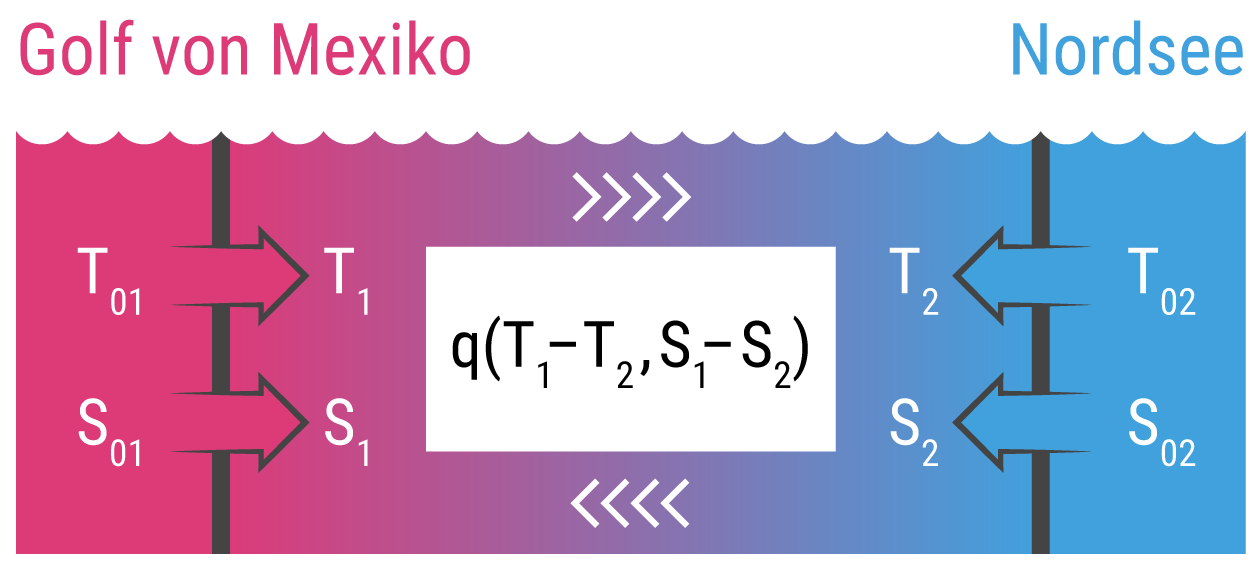
\includegraphics[width=7cm]{../Diagramme/skizze_modell.png}
  		\caption{Schematische Darstellung der zwei Behälter und des Flusses (Golfstrom) dazwischen.}
  		\label{fig:modell}
	\end{figure}
	
	Für die Indexbezeichnung der Variablen gilt in Abbildung \ref{fig:modell} sowie für das ganze nachfolgende Dokument:
	\begin{align*}
		1 &: \textrm{Golf von Mexiko} \\
		2 &: \textrm{Nordsee}
	\end{align*}

	Jeder Behälter \(i\) hat jeweils zwei sich verändernde Variablen:
	\begin{align*}
		T_i &: \textrm{Temperatur} \\
		S_i &: \textrm{Salzgehalt}
	\end{align*}
	
	Die Umgebung der Behälter wird durch folgende Konstanten beschrieben:
	\begin{align*}
		T_{0i} &: \textrm{Temperatur der Umgebung} \\
		S_{0i} &: \textrm{Salzgehalt der Umgebung}
	\end{align*}
	
	Durch das zugrunde liegende physikalische Modell \textbf{???} wird davon ausgegangen, dass sich die Behälter langsam an die Umgebungstemperatur anpassen. Also kann die Veränderung durch die Umgebungsgrößen folgendermaßen mathematisch beschrieben werden:
	\begin{align*}
		\frac{dX_i}{dt} = k_X \left( X_{0i} - X_i \right)
	\end{align*}
	Dabei ist \(X\) die zu verändernde Größe (in unserem Modell entweder \(T\) oder \(S\)).
	Die Veränderung ist also eine Zunahme der Differenz zwischen aktuellem Wert und dem Wert der Umgebung multipliziert mit einer Austauschkonstante \(k_X\).
	
	Wiederum aus dem physikalische Modell ist bekannt, dass die Veränderung durch den Fluss \(q\) sich proportional zur Differenz der Dichte der beiden Behälter beschreiben lässt:
	\begin{align*}
		q = a \left( \rho_2 - \rho_1 \right)
	\end{align*}
	Wie viel Meereswasser nun zwischen den zwei Behälter hin und her fließt, unterliegt sicherlich noch weiteren Umwelteinflüssen. Diese werden in der Konstante \(a\) zusammengefasst.
	
	Die Dichte ist abhängig von Temperatur und Salzgehalt des Meereswasser. Dieser Zusammenhang wird hier vereinfacht als linear angenommen:
	\begin{align*}
		\rho_i = \rho_0 - bT_i + cS_i
	\end{align*}
	
	Die Konstanten \(b\) und \(c\) sind also unveränderliche Naturkonstanten.
	
	Setzt man den Zusammenhang für die Dichte in die Gleichung für den Fluss ein:
	\begin{align*}
		q &= a \left( \rho_0 - bT_2 + cS_2 - \left( \rho_0 - bT_1 + cS_1 \right) \right) \\
		&= a \left( b\left( T_1 - T_2 \right) - c \left( S_1 - S_2 \right) \right)
	\end{align*}
	So wird ersichtlich, dass für den Fluss die Referenzdichte \(\rho_0\) keinen Einfluss hat.
	
	Alles zusammengesetzt ergibt für die vier veränderlichen Größen folgendes Gleichungssystem:
	\begin{align*}
		\frac{dT_1}{dt} &= k_T\left(T_{01} - T_1\right) + \left|q(T_1 - T_2,S_1 - T_2)\right|\left(T_2 - T_1\right) \\
		\frac{dT_2}{dt} &= k_T\left(T_{02} - T_2\right) + \left|q(T_1 - T_2,S_1 - T_2)\right|\left(T_1 - T_2\right) \\
		\frac{dS_1}{dt} &= k_S\left(S_{01} - S_1\right) + \left|q(T_1 - T_2,S_1 - T_2)\right|\left(S_2 - S_1\right) \\
		\frac{dS_2}{dt} &= k_S\left(S_{02} - S_2\right) + \left|q(T_1 - T_2,S_1 - T_2)\right|\left(S_1 - S_2\right)
	\end{align*}
	 
	 In den Gleichungen treten die abhängigen Größen jeweils immer als Differenz der beiden Behälter auf. Also kann das Modell so umgeschrieben werden, dass es nur noch von den Differenzen abhängt. Sei \(T = T_1 - T_2, T_0 = T_{01} - T_{02}\) und \(S = S_1 - S_2, S_0 = S_{01} - S_{02}\)  so ist:
	 \begin{align*}
	 	\frac{dT}{dt} = \frac{dT_1}{dt} - \frac{dT_2}{dt} &= k_T\left(T_{0} - T\right) - 2\left|q(T,S)\right|T \\
	 	\frac{dS}{dt} = \frac{dS_1}{dt} - \frac{dS_2}{dt} &= k_S\left(S_{0} - S\right) - 2\left|q(T,S)\right|S \\
	 	q(T,S) &= a\left(bT - cS\right)
	 \end{align*}
	  
	Aus der Realität \textbf{???} ist bekannt, dass die Umgebungstemperatur \(T_1\) im Golf von Mexiko höher ist als in der Nordsee \(T_2\). Auch bekannt ist, dass der Salzgehalt \(S_1\) im Golf tiefer ist als in der Nordsee \(S_2\). Es gilt also:
	\begin{align*}
		T_1 > T_2 \quad \textrm{und} \quad S_1 < S_2
	\end{align*}
	
	Mit diesen Bedingungen ergibt sich in einer ersten Simulation folgendes Bild:
	\begin{figure}[!h]
  		\centering
 		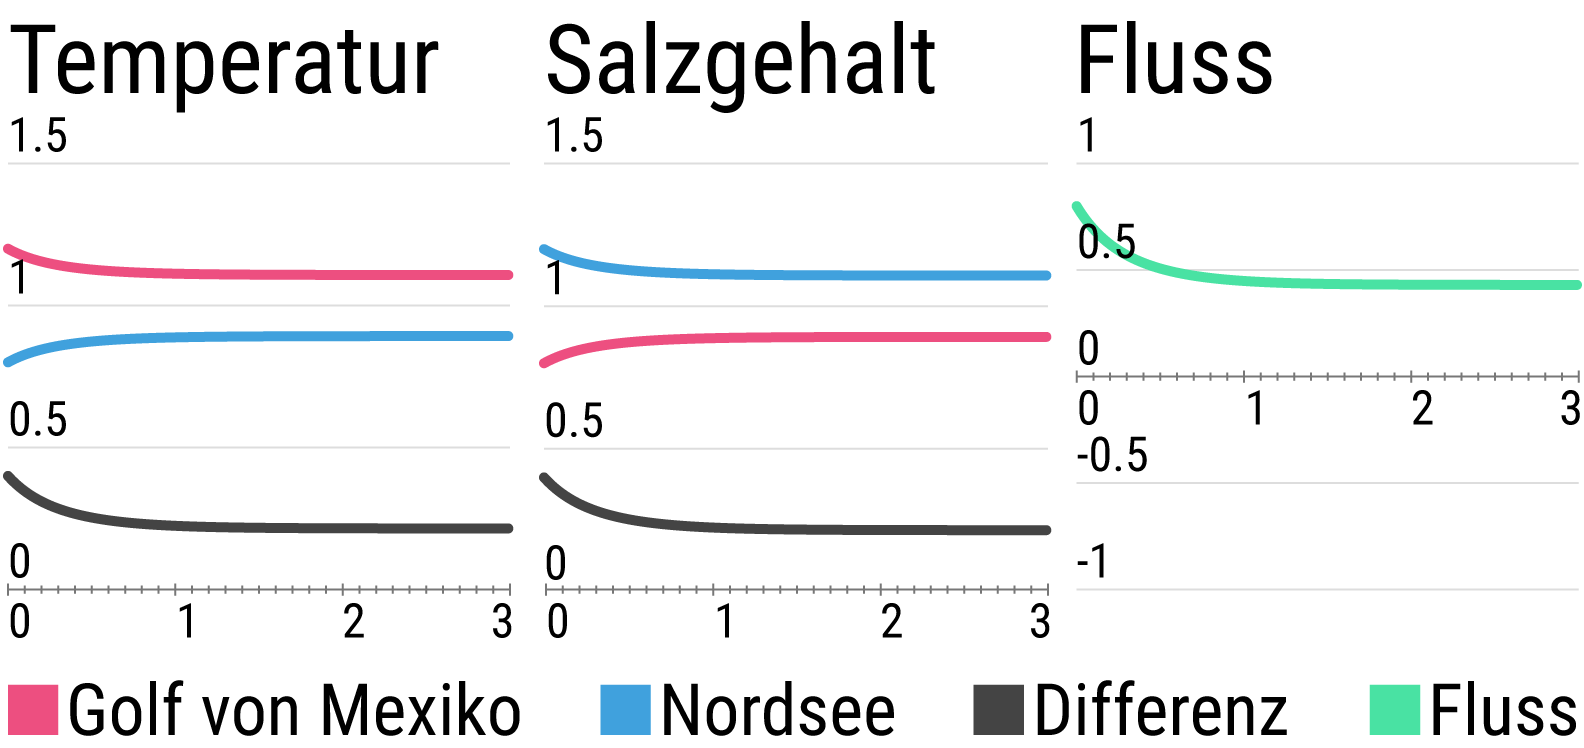
\includegraphics[width=7cm]{../Diagramme/temp-salt-flow_q-pos.png}
  		\caption{Simulation mit folgenden theoretischen Werten \(T_{01} = S_{02} = 1.2, T_{02} = S_{01} = 0.8, k_T = k_S = 1, a = b = c = 1\)}
  		\label{fig:modell_q_pos}
	\end{figure}
	
	Klar zu erkennen ist, dass sich bereits nach nur kurzer Zeit für den Fluss einen stabilen Zustand einstellt. Der Fluss stellt sich zum Ende bei \(0.45\), also fließt Wasser vom Golf von Mexiko über die Oberfläche in die Nordsee und im Untergrund wieder zurück.
	
	Sinkt der Salzgehalt in der Nordsee durch äußere Einflüsse drastisch so ergibt sich ein verändertes Bild:
	\begin{figure}[!h]
  		\centering
 		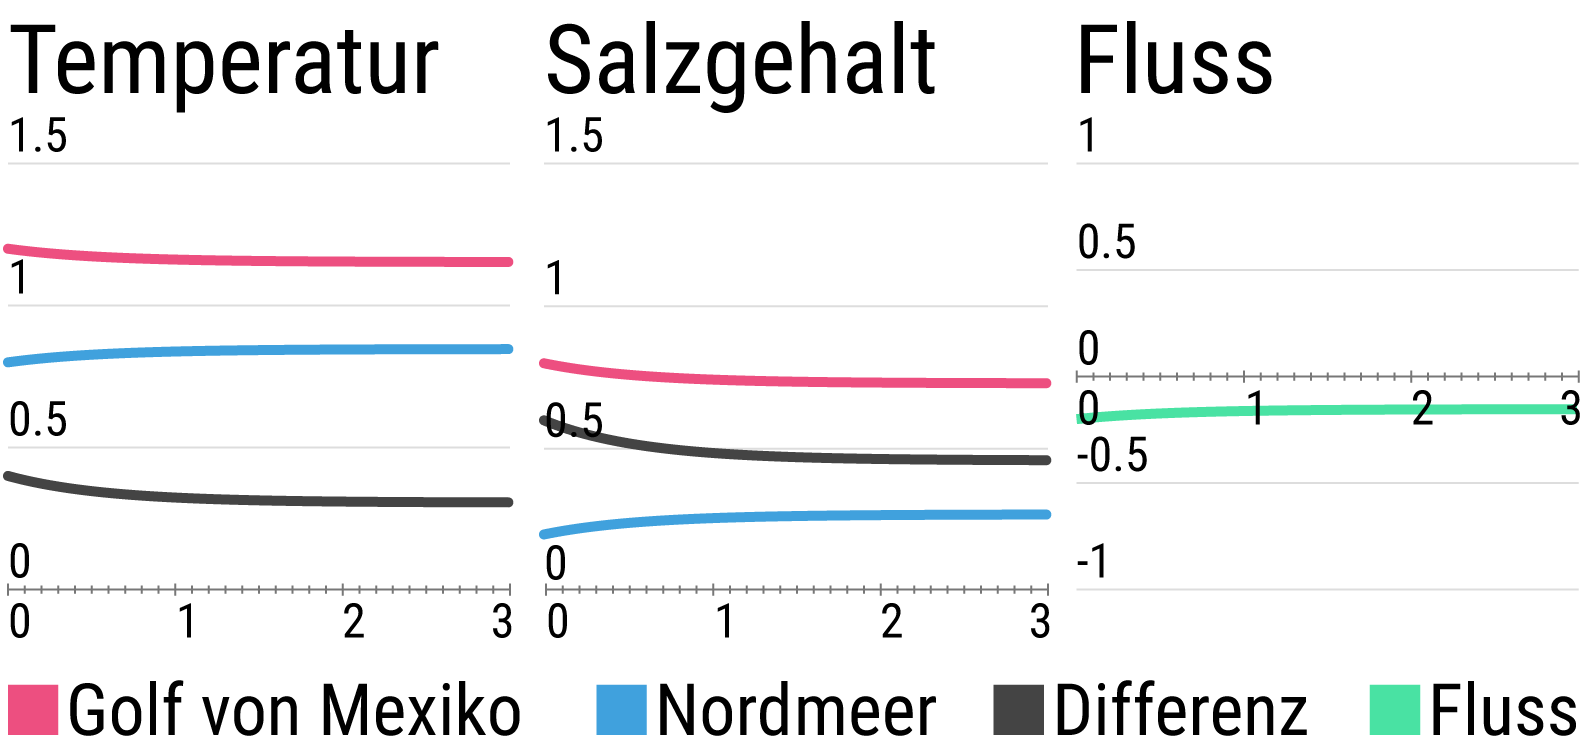
\includegraphics[width=7cm]{../Diagramme/temp-salt-flow_q-neg.png}
  		\caption{Erneute Simulation mit tiefem Salzgehalt \(S_2 = 0.2\) in der Nordsee (die anderen Parameter wurden wie in Abbildung \ref{fig:modell_q_pos} beibehalten)}
  		\label{fig:modell}
	\end{figure}
	
	In Abbildung \ref{fig:modell_q_pos} hat der Fluss ein negatives Vorzeichen, er hat sich also umgedreht. Das Wasser fließt in dieser Situation in entgegengesetzter Richtung von der Nordsee in den Golf von Mexiko.
	
	\subsection{Entdimensionalisierung}
	
	\subsection{Gleichgewichtsuntersuchung}
	
	\section{\uppercase{Anwendung}}\label{sec:Anwendung}
	
	\subsection{Datenabschätzung}
	\noindent Für Temperatur:
	% da sollte es noch was besseres geben um Links einbetten zu können?
	\begin{verbatim}
		https://www.seatemperature.org/north-sea
		https://www.seatemperature.org/mexico-sea
	\end{verbatim}
	Aber bei dieser Quelle leider keine Monatsdaten... \\
	\\
	Etwas zum Salzgehalt:
	\begin{verbatim}
		https://en.wikipedia.org/wiki/North_Sea#Temperature_and_salinity
	\end{verbatim}
	aber halt leider nur zur Nordsee \\	
	\\
	Sowas wär halt toll als Quelle:
	\begin{verbatim}
		https://data.giss.nasa.gov/
	\end{verbatim}
	Aber habe da bisher nur Daten zur Oberfächentemperatur gefunden... \\
	\\
	Vielleicht findet man da auch noch was, wenn man die Quellen durchgeht?
	\begin{verbatim}
		https://en.wikipedia.org/wiki/Sea_surface_temperature
	\end{verbatim}
	
	
	\subsection{Temperaturschwankungen durch Jahreszeiten}
	
	\subsection{Die Arktis schmilzt}
	
	\section{\uppercase{Fazit}}\label{sec:Fazit}

\end{document}	

